% uWaterloo Thesis Template for LaTeX 
% Last Updated June 14, 2017 by Stephen Carr, IST Client Services
% FOR ASSISTANCE, please send mail to rt-IST-CSmathsci@ist.uwaterloo.ca

% Effective October 2006, the University of Waterloo 
% requires electronic thesis submission. See the uWaterloo thesis regulations at
% https://uwaterloo.ca/graduate-studies/thesis.

% DON'T FORGET TO ADD YOUR OWN NAME AND TITLE in the "hyperref" package
% configuration below. THIS INFORMATION GETS EMBEDDED IN THE PDF FINAL PDF DOCUMENT.
% You can view the information if you view Properties of the PDF document.

% Many faculties/departments also require one or more printed
% copies. This template attempts to satisfy both types of output. 
% It is based on the standard "book" document class which provides all necessary 
% sectioning structures and allows multi-part theses.

% DISCLAIMER
% To the best of our knowledge, this template satisfies the current uWaterloo requirements.
% However, it is your responsibility to assure that you have met all 
% requirements of the University and your particular department.
% Many thanks for the feedback from many graduates that assisted the development of this template.

% -----------------------------------------------------------------------

% By default, output is produced that is geared toward generating a PDF 
% version optimized for viewing on an electronic display, including 
% hyperlinks within the PDF.
 
% E.g. to process a thesis called "mythesis.tex" based on this template, run:

% pdflatex mythesis	-- first pass of the pdflatex processor
% bibtex mythesis	-- generates bibliography from .bib data file(s)
% makeindex         -- should be run only if an index is used 
% pdflatex mythesis	-- fixes numbering in cross-references, bibliographic references, glossaries, index, etc.
% pdflatex mythesis	-- fixes numbering in cross-references, bibliographic references, glossaries, index, etc.

% If you use the recommended LaTeX editor, Texmaker, you would open the mythesis.tex
% file, then click the PDFLaTeX button. Then run BibTeX (under the Tools menu).
% Then click the PDFLaTeX button two more times. If you have an index as well,
% you'll need to run MakeIndex from the Tools menu as well, before running pdflatex
% the last two times.

% N.B. The "pdftex" program allows graphics in the following formats to be
% included with the "\includegraphics" command: PNG, PDF, JPEG, TIFF
% Tip 1: Generate your figures and photos in the size you want them to appear
% in your thesis, rather than scaling them with \includegraphics options.
% Tip 2: Any drawings you do should be in scalable vector graphic formats:
% SVG, PNG, WMF, EPS and then converted to PNG or PDF, so they are scalable in
% the final PDF as well.
% Tip 3: Photographs should be cropped and compressed so as not to be too large.

% To create a PDF output that is optimized for double-sided printing: 
%
% 1) comment-out the \documentclass statement in the preamble below, and
% un-comment the second \documentclass line.
%
% 2) change the value assigned below to the boolean variable
% "PrintVersion" from "false" to "true".

% --------------------- Start of Document Preamble -----------------------

% Specify the document class, default style attributes, and page dimensions
% For hyperlinked PDF, suitable for viewing on a computer, use this:
\documentclass[letterpaper,12pt,titlepage,oneside,final]{book}
 
% For PDF, suitable for double-sided printing, change the PrintVersion variable below
% to "true" and use this \documentclass line instead of the one above:
%\documentclass[letterpaper,12pt,titlepage,openright,twoside,final]{book}

% Some LaTeX commands I define for my own nomenclature.
% If you have to, it's better to change nomenclature once here than in a 
% million places throughout your thesis!
\newcommand{\E}{\mathbb{E}}
\renewcommand{\Pr}{\mathbb{P}}

\newcommand{\fracM}{\frac{1}{M}}
\newcommand{\fracMM}{\frac{1}{M^2}}
\newcommand{\sumM}{\sum_{i=1}^M}

\newcommand{\fracN}{\frac{1}{N}}
\newcommand{\fracNN}{\frac{1}{N^2}}
\newcommand{\sumN}{\sum_{j=1}^N}

\newcommand{\fracG}{\frac{1}{\Gamma}}
\newcommand{\sumG}{\sum_{i=1}^\Gamma}

\newcommand{\rhoh}{\hat{\rho}}
\newcommand{\Lh}{\hat{L}}
\newcommand{\betah}{\hat{\beta}}

\newcommand{\Bias}{\textnormal{Bias}}
\newcommand{\Variance}{\textnormal{Variance}}

% This package allows if-then-else control structures.
\usepackage{ifthen}
\newboolean{PrintVersion}
\setboolean{PrintVersion}{false} 
% CHANGE THIS VALUE TO "true" as necessary, to improve printed results for hard copies
% by overriding some options of the hyperref package below.

%\usepackage{nomencl} % For a nomenclature (optional; available from ctan.org)
\usepackage{amsmath,amssymb} % Lots of math symbols and environments
\usepackage[pdftex]{graphicx} % For including graphics N.B. pdftex graphics driver
\usepackage{booktabs}
\usepackage{amsfonts}
\usepackage{mathtools}
\usepackage{color}
\usepackage{algorithm}
\usepackage{algpseudocode}
\usepackage{algorithmicx}
\usepackage{bbm}
\usepackage{xcolor}
\usepackage{subcaption}
\usepackage{natbib}

\usepackage{tikz}
\usetikzlibrary{decorations.pathreplacing}

% Declare short-hand notations
\newtheorem{theorem}{Theorem}
\newtheorem{assumption}{Assumption}
\newtheorem{proposition}{Proposition}

\DeclarePairedDelimiter\ceil{\lceil}{\rceil}
\DeclarePairedDelimiter\floor{\lfloor}{\rfloor}

\newcommand{\SNS}{\text{SNS}}
\newcommand{\REG}{\text{REG}}
\newcommand{\KS}{\text{KS}}
\newcommand{\LR}{\text{LR}}
\newcommand{\KRR}{\text{KRR}}
\newcommand{\MSE}{\text{MSE}}

\newcommand{\convergeD}{\xrightarrow{\mathcal{D}}}
\newcommand{\convergeP}{\xrightarrow{\mathbb{P}}}
\DeclareMathOperator*{\argmax}{arg\,max}
\DeclareMathOperator*{\argmin}{arg\,min}

% Hyperlinks make it very easy to navigate an electronic document.
% In addition, this is where you should specify the thesis title
% and author as they appear in the properties of the PDF document.
% Use the "hyperref" package 
% N.B. HYPERREF MUST BE THE LAST PACKAGE LOADED; ADD ADDITIONAL PKGS ABOVE
\usepackage[pdftex,pagebackref=false]{hyperref} % with basic options
		% N.B. pagebackref=true provides links back from the References to the body text. This can cause trouble for printing.
\hypersetup{
    plainpages=false,       % needed if Roman numbers in frontpages
    unicode=false,          % non-Latin characters in Acrobat’s bookmarks
    pdftoolbar=true,        % show Acrobat’s toolbar?
    pdfmenubar=true,        % show Acrobat’s menu?
    pdffitwindow=false,     % window fit to page when opened
    pdfstartview={FitH},    % fits the width of the page to the window
    pdftitle={uWaterloo\ LaTeX\ Thesis\ Template},    % title: CHANGE THIS TEXT!
%    pdfauthor={Author},    % author: CHANGE THIS TEXT! and uncomment this line
%    pdfsubject={Subject},  % subject: CHANGE THIS TEXT! and uncomment this line
%    pdfkeywords={keyword1} {key2} {key3}, % list of keywords, and uncomment this line if desired
    pdfnewwindow=true,      % links in new window
    colorlinks=true,        % false: boxed links; true: colored links
    linkcolor=blue,         % color of internal links
    citecolor=green,        % color of links to bibliography
    filecolor=magenta,      % color of file links
    urlcolor=cyan           % color of external links
}
\ifthenelse{\boolean{PrintVersion}}{   % for improved print quality, change some hyperref options
\hypersetup{	% override some previously defined hyperref options
%    colorlinks,%
    citecolor=black,%
    filecolor=black,%
    linkcolor=black,%
    urlcolor=black}
}{} % end of ifthenelse (no else)

\usepackage[automake,toc,abbreviations]{glossaries-extra} % Exception to the rule of hyperref being the last add-on package
% If glossaries-extra is not in your LaTeX distribution, get it from CTAN (http://ctan.org/pkg/glossaries-extra), 
% although it's supposed to be in both the TeX Live and MikTeX distributions. There are also documentation and 
% installation instructions there.

% Setting up the page margins...
% uWaterloo thesis requirements specify a minimum of 1 inch (72pt) margin at the
% top, bottom, and outside page edges and a 1.125 in. (81pt) gutter
% margin (on binding side). While this is not an issue for electronic
% viewing, a PDF may be printed, and so we have the same page layout for
% both printed and electronic versions, we leave the gutter margin in.
% Set margins to minimum permitted by uWaterloo thesis regulations:
\setlength{\marginparwidth}{0pt} % width of margin notes
% N.B. If margin notes are used, you must adjust \textwidth, \marginparwidth
% and \marginparsep so that the space left between the margin notes and page
% edge is less than 15 mm (0.6 in.)
\setlength{\marginparsep}{0pt} % width of space between body text and margin notes
\setlength{\evensidemargin}{0.125in} % Adds 1/8 in. to binding side of all 
% even-numbered pages when the "twoside" printing option is selected
\setlength{\oddsidemargin}{0.125in} % Adds 1/8 in. to the left of all pages
% when "oneside" printing is selected, and to the left of all odd-numbered
% pages when "twoside" printing is selected
\setlength{\textwidth}{6.375in} % assuming US letter paper (8.5 in. x 11 in.) and 
% side margins as above
\raggedbottom

% The following statement specifies the amount of space between
% paragraphs. Other reasonable specifications are \bigskipamount and \smallskipamount.
\setlength{\parskip}{\medskipamount}

% The following statement controls the line spacing.  The default
% spacing corresponds to good typographic conventions and only slight
% changes (e.g., perhaps "1.2"), if any, should be made.
\renewcommand{\baselinestretch}{1} % this is the default line space setting

% By default, each chapter will start on a recto (right-hand side)
% page.  We also force each section of the front pages to start on 
% a recto page by inserting \cleardoublepage commands.
% In many cases, this will require that the verso page be
% blank and, while it should be counted, a page number should not be
% printed.  The following statements ensure a page number is not
% printed on an otherwise blank verso page.
\let\origdoublepage\cleardoublepage
\newcommand{\clearemptydoublepage}{%
  \clearpage{\pagestyle{empty}\origdoublepage}}
\let\cleardoublepage\clearemptydoublepage

% List of Abbreviations (abbreviations type is built in to the glossaries-extra package)
\newabbreviation{cvar}{CVaR}{Conditional Value at Risk}
\newabbreviation{gbm}{GBM}{Geometric Brownian Motion}
\newabbreviation{ml}{ML}{Machine Learning}
\newabbreviation{sns}{SNS}{Standard Nested Simulation}
\newabbreviation{var}{VaR}{Value at Risk}

% List of Symbols
\newglossary*{symbols}{List of Symbols}
\newglossaryentry{l}
{
name={$L$},
sort={label},
type=symbols,
description={Loss random variable of a financial contract}
}
 
\makeglossaries

%======================================================================
%   L O G I C A L    D O C U M E N T -- the content of your thesis
%======================================================================
\begin{document}

% For a large document, it is a good idea to divide your thesis
% into several files, each one containing one chapter.
% To illustrate this idea, the "front pages" (i.e., title page,
% declaration, borrowers' page, abstract, acknowledgements,
% dedication, table of contents, list of tables, list of figures,
% nomenclature) are contained within the file "uw-ethesis-frontpgs.tex" which is
% included into the document by the following statement.
%----------------------------------------------------------------------
% FRONT MATERIAL
%----------------------------------------------------------------------
% T I T L E   P A G E
% -------------------
% Last updated June 14, 2017, by Stephen Carr, IST-Client Services
% The title page is counted as page `i' but we need to suppress the
% page number. Also, we don't want any headers or footers.
\pagestyle{empty}
\pagenumbering{roman}

% The contents of the title page are specified in the "titlepage"
% environment.
\begin{titlepage}
        \begin{center}
        \vspace*{1.0cm}

        \Huge
        {\bf Resilient Machine Learning Approaches for Fast Risk Evaluation and Management in Financial Portfolios and Variable Annuities}

        \vspace*{1.0cm}

        \normalsize
        by \\

        \vspace*{1.0cm}

        \Large
        Xintong Li \\

        \vspace*{3.0cm}

        \normalsize
        A thesis \\
        presented to the University of Waterloo \\ 
        in fulfillment of the \\
        thesis requirement for the degree of \\
        Doctor of Philosophy \\
        in \\
        Actuarial Science \\

        \vspace*{2.0cm}

        Waterloo, Ontario, Canada, 2025 \\

        \vspace*{0.2cm}

        \copyright\ Xintong Li, 2025 \\
        \end{center}
\end{titlepage}

% The rest of the front pages should contain no headers and be numbered using Roman numerals starting with `ii'
\pagestyle{plain}
\setcounter{page}{2}

\cleardoublepage % Ends the current page and causes all figures and tables that have so far appeared in the input to be printed.
% In a two-sided printing style, it also makes the next page a right-hand (odd-numbered) page, producing a blank page if necessary.

 
% E X A M I N I N G   C O M M I T T E E (Required for Ph.D. theses only)
% Remove or comment out the lines below to remove this page
\begin{center}\textbf{Examining Committee Membership}\end{center}
  \noindent
The following served on the Examining Committee for this thesis. The decision of the Examining Committee is by majority vote.
  \bigskip
  
%   \noindent
% \begin{tabbing}
% Internal-External Member: \=  \kill % using longest text to define tab length
% External Examiner: \>  John Smith \\ 
% \> Professor, Dept. of Philosophy of XX, University of ABC \\
% \end{tabbing} 
%   \bigskip
  
  \noindent
\begin{tabbing}
Internal-External Member: \=  \kill % using longest text to define tab length
Supervisor(s): \> Mingbin Feng \\
\> Associate Professor, Dept. of Statistics and Actuarial Science\\
\> University of Waterloo \\[1cm]
\> Tony S. Wirjanto \\
\> Professor, Dept. of Statistics and Actuarial Science \\
\> University of Waterloo \\
\end{tabbing}
  \bigskip
  
  \noindent
  \begin{tabbing}
Internal-External Member: \=  \kill % using longest text to define tab length
Internal Member: \> Mary R. Hardy \\
\> Professor, Dept. of Statistics and Actuarial Science \\
\> University of Waterloo\\[1cm]
\> Chengguo Weng \\
\> Professor, Dept. of Statistics and Actuarial Science \\
\> University of Waterloo \\
\end{tabbing}
  \bigskip
  
  \noindent
\begin{tabbing}
Internal-External Member: \=  \kill % using longest text to define tab length
Internal-External Member: \> Yuying Li \\
\> Professor, School of Computer Science \\
\> University of Waterloo \\
\end{tabbing}
  \bigskip
  
  \noindent
\begin{tabbing}
Internal-External Member: \=  \kill % using longest text to define tab length
Other Member(s): \>  Emiliano Valdez \\
\> Professor, Dept. of Mathematics \\
\> University of Connecticut \\
\end{tabbing}

\cleardoublepage

% D E C L A R A T I O N   P A G E
% -------------------------------
  % The following is a sample Delaration Page as provided by the GSO
  % December 13th, 2006.  It is designed for an electronic thesis.
  \noindent
I hereby declare that I am the sole author of this thesis. This is a true copy of the thesis, including any required final revisions, as accepted by my examiners.

\bigskip
  
\noindent
Part of the work in this thesis has been published in a Winter Simulation Conference proceeding.

  \bigskip
  
  \noindent
I understand that my thesis may be made electronically available to the public.

\cleardoublepage

% A B S T R A C T
% ---------------

\begin{center}\textbf{Abstract}\end{center}

Risk management of financial derivatives and actuarial products is intricate and often requires modeling the underlying stochasticity with Monte Carlo simulations.
Monte Carlo simulation is flexible and can easily adapt to changes in model assumptions and market conditions.
However, as multiple sources of risk are considered over long time horizons, the simulation model becomes complex and time-consuming to run.
Tremendous research effort has been dedicated to designing computationally efficient machine learning-based procedures that mitigate the computational burden of a standard simulation procedure.
In machine learning, model flexibility comes at the expense of model resilience, which is crucial for risk management tasks.
This study considers estimating tail risks of complex financial and actuarial products with resilient machine learning-based nested simulation procedures.
We propose a novel metamodeling approach that integrates deep neural networks within a nested simulation framework for efficient risk estimation.
Our approaches offer substantial improvements over the associated standard simulation procedures.
This study also illustrates how to build and assess resilient machine learning models for different problem complexities and different data structures, qualities, and quantities.
To further enhance adaptability to new variable annuity contracts and changing market conditions, this thesis explores transfer learning techniques.
By reusing and fine-tuning pre-trained metamodels, the proposed approach accelerates the adaptation process to different contract features and evolving market dynamics without retraining models from scratch.
Transfer learning improves computational efficiency and enhances the robustness and flexibility of neural network metamodels in dynamic hedging of variable annuities.

Extensive numerical experiments in this thesis demonstrate that the proposed methods substantially improve computational efficiency, sometimes shortening runtime by orders of magnitude compared to standard nested simulation procedures.
The results indicate that deep neural network metamodels with transfer learning can quickly adapt to new market scenarios and contract specifications.
This research contributes to the advancement of risk management practices for complex actuarial products and financial derivatives.
By leveraging advanced machine learning techniques, this thesis offers a practical and scalable solution for insurers to perform timely and accurate risk assessments.
The integration of long short-term memory metamodels and transfer learning into a nested simulation framework represents a major step forward toward more efficient, adaptable, and robust methodologies in actuarial science and quantitative finance.


\cleardoublepage

% A C K N O W L E D G E M E N T S
% -------------------------------

\begin{center}\textbf{Acknowledgements}\end{center}

I would like to express my deepest gratitude to Professor Mingbin Feng and Professor Tony Wirjanto for their invaluable support and guidance throughout my academic journey. 
Their unwavering patience and profound wisdom have been instrumental in helping me navigate the complexities of my research. 
I am deeply grateful for their mentorship, which has not only sharpened my analytical skills but also inspired me to pursue excellence in my work.

Additionally, I extend my sincere thanks to my best friends. 
Their unwavering support and encouragement have been a constant source of strength that has helped me overcome obstacles and maintain my motivation throughout this process. 
Words cannot fully convey how much their presence has meant to me over these years.

I also wish to acknowledge the support of my family, who have always been a source of love and encouragement.
They have provided me with the emotional stability I needed to focus on my studies and research.

\cleardoublepage

% T A B L E   O F   C O N T E N T S
% ---------------------------------
\renewcommand\contentsname{Table of Contents}
\tableofcontents
\cleardoublepage
\phantomsection    % allows hyperref to link to the correct page

% L I S T   O F   T A B L E S
% ---------------------------
\addcontentsline{toc}{chapter}{List of Tables}
\listoftables
\cleardoublepage
\phantomsection		% allows hyperref to link to the correct page

% L I S T   O F   F I G U R E S
% -----------------------------
\addcontentsline{toc}{chapter}{List of Figures}
\listoffigures
\cleardoublepage
\phantomsection		% allows hyperref to link to the correct page

% GLOSSARIES (Lists of definitions, abbreviations, symbols, etc. provided by the glossaries-extra package)
% -----------------------------
\printglossaries
\cleardoublepage
\phantomsection		% allows hyperref to link to the correct page

% Change page numbering back to Arabic numerals
\pagenumbering{arabic}

 

%----------------------------------------------------------------------
% MAIN BODY
%----------------------------------------------------------------------
% Because this is a short document, and to reduce the number of files
% needed for this template, the chapters are not separate
% documents as suggested above, but you get the idea. If they were
% separate documents, they would each start with the \chapter command, i.e, 
% do not contain \documentclass or \begin{document} and \end{document} commands.

%======================================================================
\chapter{Introduction}
%======================================================================

Quantitative risk management is a key component of modern financial systems.
Successful risk management practice ensures the stability and resilience against a variety of risks.
For financial products like option portfolios and variable annuity (VA) contracts, traditional risk assessment methods often fall short in accurately capturing the complex dynamics of the underlying risk factors.
VA contracts are a popular type of complex insurance product that is linked to the performance of underlying assets.
It provides a guaranteed minimum income benefit to the policyholder regardless of the performance of the underlying assets.
Advanced Monte Carlo simulation techniques, particularly nested simulation procedures, become indispensable for risk assessment of such products.
In contrast to finite-difference methods, a Monte Carlo simulation scheme is more flexible and can be easily adapted to model tail risk with a rule-based design.
~\cite{glasserman2004monte} provide a comprehensive overview of Monte Carlo simulation methods in financial engineering and risk management applications.
In this thesis, we focus on building and analyzing nested simulation procedures for risk management applications of financial derivatives and insurance products.
Nested simulation, also known as nested stochastic modeling and stochastic-on-stochastic modeling, becomes necessary when stochastic simulation of a parameter of interest is contingent on another quantity to be determined stochastically.
In the context of financial engineering, nested simulation is used to model the tail risk of a contract whose payoff depends on a set of underlying risk factors.
For example, estimating the value of an exotic option at a risk horizon requires simulation given a realization of the underlying assets upto that horizon.
A standard nested simulation procedure consists of two levels of simulation: the outer-level simulation generates the underlying risk factors, while the inner-level simulation estimates the value of interest with the inner sample mean from another level of Monte Carlo simulation.
This nested structure allows for accurate estimation given sufficient computational resources, but it also introduces additional complexity in the simulation design and implementation.
Furthermore, in real-world applications, the computational burden of nested simulation can be prohibitive.
The number of inner simulations required to achieve a desired level of accuracy for each outer scenario can be infeasibly large.
Metamodeling techniques that approximate the inner simulation model can be used to reduce the computational burden of nested simulation.
Metamodels are statistical models that approximate the output of a complex simulation model as a function of its input parameters.
In this thesis, we focus on metamodels of the inner simulation models in nested simulation procedures for risk management applications of financial derivatives and VA contracts.
Two interesting problems that requires nested simulation are considered in this thesis:  
\begin{itemize}
    \item estimating the risk of a portfolio of financial options and 
    \item dynamic hedging of VA contracts with a delta hedging strategy.
\end{itemize}
The risk management of VAs is a challenging problem due to the complex interactions between the policyholder's behavior, the financial market dynamics, and the insurer's risk management strategies.
We focus mainly on the estimation of tail risk measures of VA contract losses using metamodel-based nested simulation procedures.
This thesis consists of four chapters. 
Chapter \ref{chap:project1} summarizes theoretical convergence results of several state-of-the-art single-period nested simulation procedures under the same analytical framework. 
Numerical experiments are conducted to test their empirical convergence behavior under finite budget sizes.
Chapter~\ref{chap:project2} proposes the use of neural network models as metamodels for a two-stage multi-period nested simulation procedure on VA contracts. 
In our numerical experiment, the best neural network metamodel surpasses the state-of-the-art metamodels in tail identification, and it leads to substantial computational savings. 
Chapter~\ref{chap:project2} also conducts sensitivity testing on the neural network metamodel. 
We argue that for estimating tail risk measures of VA contact losses, the inner simulation can be replaced entirely by a suitable metamodel. 
Eliminating the inner simulation can lead to more substantial computational savings without affecting estimation quality. 
In the case of requiring extensive inner simulations for regulatory purposes, effective budget allocations can help achieve higher estimator quality with the same computational budget.
In practice, underlying assumptions of the simulation model are subject to change, and new VA contracts are issued with different contract specifications.
Simulation budgets are often scarce for new conditions.
Chapter~\ref{chap:project3} uses transfer learning techniques for quick adaptation of the neural network metamodel to new market conditions and new VA contracts.
Our numerical experiments shows that an intelligent use of transfer learning can lead to significantly better metamodels than those trained from scratch.
Chapter~\ref{chap:futureWork} discusses the application of deep reinforcement learning in the dynamic hedging of VA contracts.
Chapter \ref{chap:conclusion} concludes the thesis and discusses potential future research directions.

\section{Managing Risk of Variable Annuity with Nested Simulation}

VA contracts are index-linked insurance products that offer policyholders the upside potential of equity markets while providing guarantees that protect against downside risk.
These products have gained significant interest as they address the needs of individuals seeking both wealth accumulation and financial security, especially in the context of retirement planning.
The most interesting feature of VAs is embedded guarantees that ensure a specified minimum benefit regardless of market performance.
Two VA contracts that are most relevant to this thesis are Guaranteed Minimum Maturity Benefit (GMMB) and the Guaranteed Minimum Withdrawal Benefit (GMWB). 
The GMMB guarantees that at the maturity of the contract, the policyholder will receive no less than the initial investment or a predetermined minimum amount. 
The GMWB allows policyholders to withdraw a specified percentage of their benefit base each period during the contract horizon~\citep{hardy2003investment}.
While these guarantees enhance the attractiveness of VAs to consumers by offering protection against market downturns and ensuring income stability, they introduce substantial financial risks to insurers. 
The embedded options within GMMBs and GMWBs expose insurers to market risk, longevity risk, and policyholder behavior risk. 
Effective management of these risks is crucial for insurers to maintain solvency and meet regulatory capital requirements.

One of the primary risk management strategies employed by insurers to mitigate the financial risks associated with VAs is dynamic hedging. 
Dynamic hedging involves frequently adjusting a portfolio of financial instruments to offset changes in the value of the guarantees due to market movements~\citep{hull2016options}. 
This strategy aims to neutralize the sensitivity of the insurer's liability to market fluctuations by constructing a hedging portfolio that replicates the cash flows of the guarantees.
However, dynamic hedging introduces complexity in estimating the insurer's overall risk exposure.
One of such examples is the estimation of tail risk measures of a VA contract.
It requires the stochastic modeling of the financial market and the accurate loss estimation of the hedging portfolio under different market scenarios.
Nested simulation has emerged as a robust method for estimating risk measures in such complex settings~\citep{gordy2010nested}.
In nested simulation, an outer simulation generates a set of market scenarios over the contract horizon, while an inner simulation estimates the contract loss in each scenario.
By combining the results of the inner simulations across the outer scenarios, nested simulation provides an accurate estimate of the tail risk of the VA contract.

Despite its robustness, nested simulation is computationally intensive, often requiring significant computational resources and time. 
Each scenario in the outer simulation requires numerous inner simulations to accurately estmate contract loss. 
This computational burden poses practical limitations, especially when high precision in tail risk estimation is required.
To address this challenge, metamodeling techniques can be employed to approximate the inner simulation model and reduce the computational cost of nested simulation.

\section{Metamodeling for Monte Carlo Simulation}

Metamodeling, also known as surrogate modeling, is a technique used to approximate complex simulation models with simpler, computationally efficient models. 
In the context of Monte Carlo simulations, metamodels are models of models that aim to reduce computational costs by creating an approximate model that can quickly predict simulation outputs based on input variables~\citep{kleijnen2018design}. 
This section introduces metamodeling for Monte Carlo simulation, elaborates on its methodologies, and highlights its importance in practical applications.

Monte Carlo simulations are widely used for modeling and analyzing complex systems that are probabilistic in nature. 
These simulations often require a significant amount of computational resources, especially when high accuracy or numerous iterations are necessary~\citep{glasserman2004monte}. 
Metamodeling addresses this challenge by constructing an approximate model (metamodel) that emulates the behavior of the original simulation model with much less computational effort.
The metamodel serves as a predictive model that maps input variables to output responses. 
Learning from a set of simulation runs, the metamodel can generalize and predict outputs for new inputs without running the full simulation.
Metamodeling is particularly useful when the simulation model is computationally expensive. 
By replacing the simulation model with a metamodel, the computational cost of evaluating the model can be significantly reduced. 
This allows for faster convergence of simulation-based estimators.

The process of metamodeling generally involves:

\begin{enumerate} 
    \item \textbf{Design of Experiments}: Selecting input combinations to run the original simulation and collect data. 
    \item \textbf{Building the Metamodel}: Using the collected data to train a metamodel that approximates the simulation model. 
    \item \textbf{Validation}: Assessing the metamodel's accuracy and generalization capability.
    \item \textbf{Application}: Using the metamodel to predict simulation outputs for new input combinations.
\end{enumerate}

The development of advanced machine learning models and deep learning techniques has significantly enhanced metamodeling approaches for Monte Carlo simulations, especially in high-dimensional and complex problem settings.
Example use cases for machine learning include~\cite{jin2020deep}, ~\cite{tang2020deep}, and~\cite{rosen2012metamodeling}.
These methods offer powerful tools for capturing intricate patterns and nonlinear relationships that traditional metamodeling techniques might struggle to model effectively.
In the following sections, we discuss machine learning algorithms in the context of metamodeling for Monte Carlo simulations and their applications in risk management.

\section{Machine Learning for Risk Management Applications}

Machine learning (ML) algorithms are essential tools for identifying complex patterns and relationships in data. 
In particular, they are well-suited for handling non-linearities and large-scale data structures, which are challenging for traditional statistical methods. 
In the context of risk management, ML algorithms have been widely used for predicting financial time series, estimating risk measures, and optimizing trading strategies.
ML algorithms can be broadly categorized into supervised learning, unsupervised learning, and reinforcement learning.
This section focuses on three widely used supervised learning models and two reinforcement learning algorithms that are relevant to risk management applications.

\subsection{Supervised Learning Models}

Supervised learning is a fundamental approach in machine learning where the algorithm learns a mapping from inputs to outputs based on example input-output pairs \cite{galton1886regression}. 
In this paradigm, a model is trained on a labeled dataset, which means that each training example is associated with an output label or value. 
The goal is to learn a general rule that maps inputs (also known as features) to outputs (also known as target), enabling the model to make accurate predictions on new, unseen data.

\begin{itemize} 
    \item \textbf{Classification}: The output variable is categorical, and the task is to assign inputs to one of several predefined categories. 
    Common use in finance and actuarial applications are fraud detection and credit scoring.
    \item \textbf{Regression}: The output variable is continuous, and the task is to predict a real-valued number. 
    Examples in actuarial applications include predicting claim amounts, reserve estimates, asset pricing, and estimating tail risk measures of loss distributions.
\end{itemize}

This thesis focuses on regression models for risk management applications, where the goal is to predict a continuous target variable based on one or more input features.
Given a dataset of $n$ observations $\{(x_1, y_1), (x_2, y_2), \ldots, (x_n, y_n)\}$, where $x_i \in \mathbb{R}^d$ is the $d$-dimensional input feature vector, and $y_i \in \mathbb{R}$ is the target variable, a supervised learning algorithm aims to learn a function $f(;\theta): \mathbb{R}^d \rightarrow \mathbb{R}$ that best predicts the target variable $y$ given the input features $x$ with a set of function parameters $\theta$.

Linear regression, kernel regression, and neural networks all fall under the supervised learning category and are widely used in risk management applications.
Despite the differences in their functional forms, all supervised learning models can be evaluated on a similar set of metrics.
The learning process is referred to as training, which involves minimizing a loss function $l(f(x; \theta),y)$ over the training data, which quantifies the difference between the predicted labels and the training labels.
A common loss function for regression problems is the mean squared error (MSE):

\begin{equation} \label{eq:mse}
    \text{MSE} = \frac{1}{n} \sum_{i=1}^{n} (f(x_i;\theta) - y_i)^2.
\end{equation}

In most risk management applications, a critical task of users of supervised learning models is to design a suitable loss function that aligns with the objectives of the problem.
Another important consideration is the choice of a suitable supervised learning algorithm.
The choice may vary based on the complexity of the relationship, the interpretability of the model, and the computational resources available.
In the following sections, we discuss four widely used supervised learning techniques in risk management applications: parametric regression, kernel regression, and two neural network architectures.

\subsection{Parametric Regression Models}

Regression models are the most common supervised learning algorithms used in risk management applications.
A regression model predicts a continuous target variable based on one or more input features.
Linear regression is a simple and interpretable model that attempts to predict a target variable as a linear combination of input features. 
It assumes a linear relationship between the target output and one or more input features. 
This method has been thoroughly explored in statistical literature. 
\citet{bishop2006pattern} provide an extensive treatment of regression techniques in the broader context of machine learning.
It is known as parametric regression because it assumes a specific functional form for the input-output relationship with a finite set of parameters~\citep{seber2012linear}.
General form of a parametric regression model is given by:
\begin{equation} \label{eq:regression}
    f(x; \theta) = \beta_0 + \sum_{j=1}^{p} \beta_j \phi_j(x),
\end{equation}
where $p$ is the number of features, $\beta_0, \beta_1, \ldots, \beta_p$ are the trainable regression coefficients, and $\phi_j(x)$ are basis functions that transfrom the input $x$ to allow for non-linear modeling.
Basis functions can be any functions of $x$ that are chosen to capture the underlying structure of the data.
Common choices include polynomial basis functions: $\phi_j(x) = x^j$ and Laguerre basis functions: $\phi_j(x) = e^{-x/2} L_j(x)$, where $L_j(x)$ are the Laguerre polynomials that are solutions to the Laguerre differential equation~\citep{szeg1939orthogonal}.
The training of parametric regression refers to the process of estimating the regression coefficients $\beta_0, \beta_1, \ldots, \beta_p$ that minimize the loss function.
For a MSE loss, the optimal regression coefficients can be obtained by solving the normal equations.
Parametric regression is a powerful tool for modeling linear relationships where the basis functions are known from expert knowledge for explicit feature engineering techniques~\citep{hastie2009elements}.
These techniques utilize predefined functional forms to model the relationship between independent variables and the dependent variable. 
However, when data exhibits complex, non-linear relationships, linear models fall short. 
While these methods are straightforward and interpretable, they impose strong assumptions about the underlying data structure.
Often, expert knowledge is required to select the appropriate basis functions, which can limit the flexibility of the model.
Extensions like polynomial regression and generalized linear models (GLMs) have been introduced to capture non-linearity.
Nevertheless, these models can still be limited in capturing highly complex patterns. 

\subsection{Non-Parametric Regression Models}
To overcome some limitations of parametric regression, non-parametric methods such as kernel regression~\citep{hastie2009elements} are often employed. 
Kernel regression estimates the relationship by averaging the values of the target variable over a local neighborhood of the input $x$.
The kernel regression with the Nadaraya-Watson estimator is given by:
\begin{equation}
    f(x; \theta) = \frac{\sum_{i=1}^{n} K\left(\frac{x-x_i}{h}\right) y_i}{\sum_{i=1}^{n} K\left(\frac{x-x_i}{h}\right)},
\end{equation}
where $K(\cdot)$ is the kernel function, which assigns weights to the data points based on their distance to the input $x$, and $h$ is the bandwidth parameter that controls the smoothness of the estimated function.
The objective is to estimate the feature-label relationship directly from the data without imposing a specific form.
However, they come with several drawbacks that limit their effectiveness, especially in high-dimensional settings or for large datasets. 
One of the most significant drawbacks of non-parametric regression is the curse of dimensionality \cite{bellman1966dynamic}. 
As the number of features increases, the volume of the input space grows exponentially.
Data points become sparse and the model may overfit to noise in the data.
In addition, the computational cost associated with non-parametric methods often grows rapidly with the number of dimensions.
Cross validation and distance calculation are two computationally expensive operations that are often required for non-parametric regression.
These drawbacks make non-parametric regression impractical for modeling high-dimensional large-scale datasets. 

\subsection{Feedforward Neural Networks}

The progression from traditional parametric and non-parametric regression methods to neural network architectures has been driven by the need to model increasingly complex and high-dimensional data.
Neural networks have emerged as powerful tools capable of overcoming many limitations of traditional regression methods. 
They can learn complex, non-linear relationships in data without the need for explicit feature engineering.
The most crude form of a neural network is the feedforward neural network (FNN), which consists of an input layer, one or more hidden layers, and an output layer~\citep{goodfellow2016}.

\begin{figure}[ht!]
    \centering
    \begin{subfigure}{0.45\textwidth}
        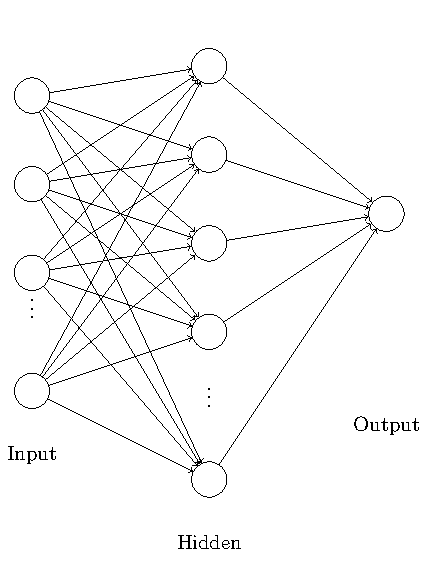
\includegraphics[width=\textwidth]{./project3/tikz/fnn.pdf}
        \caption{FNN}
        \label{subfig:fnn}
    \end{subfigure}
    \hspace{1cm}
    \begin{subfigure}{0.45\textwidth}
        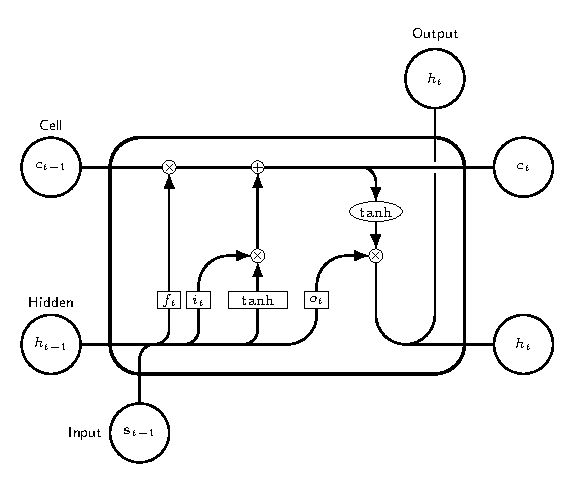
\includegraphics[width=\textwidth]{./project3/tikz/lstm.pdf}
        \caption{LSTM}
        \label{subfig:lstm}
    \end{subfigure}
    \caption{Neural Network Architectures}
    \label{fig:nn}
\end{figure}

Figure~\ref{subfig:fnn} shows a feedforward neural network (FNN) architecture with one hidden layer.
The input layer receives the input features, which are then passed through the hidden layer(s) to the output layer.
Each layer consists of multiple neurons, which apply a non-linear activation function to the weighted sum of the inputs.

\begin{equation}
    f(x; \theta) = f^{(k)}(f^{(k-1)} \cdots (f^{(2)}(f^{(1)}(x;\theta^{(1)});\theta^{(2)} )\cdots ;\theta^{(k-1)});\theta^{(k)}),
\end{equation}

where $\theta = (\theta^{(1)}, \theta^{(2)}, \ldots, \theta^{(k)})$ are the trainable parameters of the neural network, $f^{(i)}$ is the $i$-th layer of the neural network, $x$ is the input feature vector, $f^{(1)}(x;\theta^{(1)}) = x$, $f^{(k)}$ is the output layer, $k$ is the number of layers, and $f^{(i)}$ is the output of the $i$-th layer.
To move from a lower layer to a higher layer, i.e., from layer $i-1$ to layer $i$,

\begin{equation} \label{eq:neural}
    f^{(i)}(z;\theta^{(i)}) = a^{(i)}(\beta_0^{(i)} + \sum_{j=1}^{p_i} \beta_j^{(i)} z),
\end{equation}

where $a^{(i)}$ are the nonlinear activation functions, $\theta^{(i)} = (\beta_0^{(i)}, \dots, \beta_p^{(i)})$ are the trainable parameters of the $i$-th layer, and $p_i$ is the number of neurons in the previous layer.
Equation~\ref{eq:neural} represents a single neuron in a neural network, which applies a linear transformation to the input followed by a non-linear activation function. 
The linear transformation is similar to the linear regression model in Equation~\ref{eq:regression}, but the non-linear activation function allows the neural network to model complex, non-linear relationships in the data.
The FNN is tuned by adjusting the trainable parameters $\theta$ while fixing the activation functions $a^{(i)}$.
A typical choice for the activation function is the rectified linear unit (ReLU), which is defined as $a(z) = \max(0, z)$~\citep{nair2010rectified}.
The choice of activation function also plays a crucial role in the training of neural networks.
While sigmoid and hyperbolic tangent functions were popular in early neural networks, ReLU has become the default activation function for deep networks due to its ability to mitigate the vanishing gradient problem and promote sparse activations~\citep{lecun2015deep}.

The key advantage of feedforward neural networks (FNNs) lies in their ability to perform automatic feature engineering without direct human intervention. 
Unlike traditional machine learning models that require manual selection and transformation of input features, neural networks learn to extract and compose features through their hidden layers during the training. 
Each hidden layer in the network captures higher-level abstractions of the input data by transforming the outputs of the previous layer through nonlinear activation functions~\citep{lecun2015deep}.
Each layer builds upon the representations learned by the previous layer, enabling the network to capture multiple levels of abstraction. 
This characteristic is crucial for modeling complex datasets with intricate patterns and relationships~\citep{bengio2013representation}.

The last layer of the neural network, known as the output layer, typically performs a linear transformation of the features extracted by the preceding hidden layers. 
With $a^{k}(z) = z$, the last layer is equivalent to a linear regression with its inputs as transformed, high-level features learned by the hidden layers.
We can draw parallels between neural networks and traditional regression models. 
The main difference is that, in neural networks, the input features to the regression model are learned automatically rather than being manually specified.

The most well-known theorem in neural network theory is the universal approximation theorem~\citep{hornik1989multilayer}.
It states that given appropriate activation functions $a$, a feedforward neural network with a single hidden layer containing a finite number of neurons can approximate any continuous function on a compact subset of $\mathbb{R}^n$ to arbitrary accuracy. 
Despite this theoretical guarantee for single-layer neural networks, in practice, deep neural networks (DNN) with multiple hidden layers have been shown to be more effective at capturing complex patterns and relationships in data~\citep{lecun2015deep}.
Examples include AlexNet~\citep{krizhevsky2012imagenet}, VGG~\citep{simonyan2014very}, and ResNet~\citep{he2016deep}, which have achieved state-of-the-art performance on image classification tasks.
In this thesis, we focus on the application of deep neural networks, specifically long short-term memory (LSTM) networks, as metamodels for nested simulation procedures in risk management applications.

\subsection{Training and Evaluation of Neural Networks}

The training of neural networks involves adjusting the trainable parameters of the network to minimize the loss function, which quantifies the error between the predictions and labels.
The training process aims to find the optimal parameters that minimize this error.
The most common approach is to use gradient descent methods with backpropagation, which is an efficient method for computing the gradients of the loss function with respect to the trainable parameters.
Backpropagation computes the gradients by propagating the error derivatives backward through the network layers.
This process allows the network to adjust the parameters in the direction of minimizing the loss function.
The training process is typically performed over a number of epochs, where each epoch is one complete pass through the training dataset.

However, the training of neural networks is non-convex, and the optimization problem is challenging.
Stochastic gradient descent (SGD) is a popular optimization algorithm for training neural networks.
It updates the parameters using a single or a small batch of training examples at a time, which makes it much faster than the crude gradient descent.
However, SGD may oscillate and converge slowly, especially in non-convex problems~\citep{bengio2016}.
To address these issues, various adaptive learning rate methods have been proposed.
The most popular approach is Adam, which is a SGD algorithm that adjusts the learning rate during training to improve convergence speed and stability~\citep{kingma2014adam}.

Another common technique to improve the training of neural networks is regularization to prevent overfitting.
One effective regularization method is dropout, which randomly sets a fraction of neurons to zero during each training iteration~\citep{srivastava2014dropout}.
This prevents neurons from co-adapting too much, encourages redundancy, and leads to a more robust model that generalizes better to unseen data.
Early stopping is another regularization method that is relevant to our study.
It involves monitoring the model's performance on a validation set and stopping training when the performance no longer improves~\citep{prechelt2002early}.
This helps prevent over-fitting by stopping training before the model begins to fit to noise in the data.

Evaluation of the performance of a neural network is challenging due to the absence of analytical tools.
Existing machine learning literature addresses this challenge by splitting the data into three parts: training set, validation set, and test set.
The training set is used to train the model, the validation set is used to tune the model hyper-parameters, and the test set is used to evaluate how well the model generalizes to unseen data.
The test set is not used during training and is only used for evaluation.

Under-fitting occurs when the training error is high, which means that the neural network fails to capture the underlying patterns in the training data.
Over-fitting occurs when the neural network fits to noise in the training data and cannot generalize to unseen data.
In machine learning literature, over-fitting is often quantified as the gap between the training error and the test error~\citep{bishop2006pattern}.
During training, as the test dataset is not used, this quantity is estimated using the validation set.
If the validation error is high compared to the training error, the model is likely over-fitting to the training data.

\subsection{Long Short-Term Memory Networks}

Building upon the capabilities of FNNs, we recognize that while FNNs are successful at capturing complex, nonlinear relationships through automatic feature learning, they are inherently limited when it comes to modeling sequential data or time-dependent patterns. 
This independence assumption limits their effectiveness in modeling financial time series, where temporal dependencies play a critical role. 
The stylized facts of financial time series, such as volatility clustering, fat tails, and autocorrelation, are challenging to capture with traditional FNNs due to the absence of memory in the model~\citep{cont2001empirical}.

To overcome the limitations of FNNs in handling sequential input, recurrent neural networks (RNNs) were introduced.
In a RNN, the hidden state at each time step is a function of both the current input and the hidden state from the previous time period~\citep{elman1990finding}:

\begin{equation}
    h_t = f(x_t, h_{t-1}; \theta),
\end{equation}

where $h_t$ is the hidden state at time $t$, $x_t$ is the input at time $t$, $h_{t-1}$ is the hidden state at time $t-1$, and $f$ is the recurrent function parameterized by $\theta$.
This architecture enables RNNs to capture temporal dependencies by maintaining a dynamic internal state that reflects the memory of past inputs.
However, traditional RNNs suffer from the vanishing and explodeing gradient problem, which hinders their ability to capture long-term dependencies that often present in financial time series~\citep{bengio1994learning}.
During training, gradients propagated backward through time can either diminish exponentially (vanishing gradients) or grow uncontrollably (exploding gradients).
This limitation is particularly problematic in modeling long-term financial contracts and insurance guarantees, where patterns may span over extended periods.

To address these issues, a long short-term memory (LSTM) network was developed by \citet{hochreiter1997long}.
It is a specialized form of RNNs designed to capture long-term dependencies more effectively with the help of RNN memory cells and gating mechanisms.

\begin{align*}
    i_t &= a(W_i x_t + U_i h_{t-1} + b_i), \\
    f_t &= a(W_f x_t + U_f h_{t-1} + b_f), \\
    o_t &= a(W_o x_t + U_o h_{t-1} + b_o), \\
    g_t &= a(W_g x_t + U_g h_{t-1} + b_g), \\
    c_t &= f_t \odot c_{t-1} + i_t \odot g_t, \\
    h_t &= o_t \odot \tanh(c_t),
\end{align*}

where $i_t, f_t, o_t, g_t, c_t, h_t$ are the input gate, forget gate, output gate, cell input, cell state, and hidden state at time $t$, respectively.
$W_i$, $W_f$, $W_o$, $W_g$, $U_i$, $U_f$, $U_o$, $U_g$ are the weight matrices, and $b_i$, $b_f$, $b_o$, $b_g$ are the bias vectors.
$a$ is the activation function, typically the sigmoid function, and $\odot$ denotes element-wise multiplication.

\begin{equation*}
    a(z) = \frac{1}{1 + e^{-z}}.
\end{equation*}

Figure~\ref{subfig:lstm} shows the architecture of an LSTM network.
The gating mechanisms in LSTM networks effectively mitigate the vanishing and exploding gradient problem by regulating the flow of information through the network.
The input gate $i_t$ controls the flow of information into the cell state $c_t$, the forget gate $f_t$ regulates the retention of information in the cell state, and the output gate $o_t$ determines the information passed to the hidden state $h_t$.
The cell input $g_t$ is used to update the cell state based on the input $x_t$ and the previous hidden state $h_{t-1}$.
The cell state $c_t$ acts as a memory unit that stores information over time, while the hidden state $h_t$ captures the relevant information for the current time step.
By incorporating memory cells and gating mechanisms, LSTMs can effectively model long-term dependencies in sequential data in finance and actuarial applications.

The advancements in neural network optimization techniques, architectures, and training methodologies have significantly enhanced their usefulness in risk management applications.
By effectively modeling complex, non-linear relationships and temporal dependencies, neural networks serve as powerful tools for addressing the computational challenges in estimating risk measures and developing effective risk mitigation strategies.
This thesis aims to explore the application and noise tolerance of LSTM networks in metamodeling for nested simulation procedures in risk management.
We investigate the performance of LSTM networks in approximating the inner simulation model in a two-stage nested simulation procedure for index-linked insurance contracts.
By leveraging the memory and sequential modeling capabilities of LSTMs, we aim to improve the accuracy and efficiency of nested simulation procedures for risk management applications.


%----------------------------------------------------------------------
% END MATERIAL
%----------------------------------------------------------------------

% B I B L I O G R A P H Y
% -----------------------

% The following statement selects the style to use for references.  It controls the sort order of the entries in the bibliography and also the formatting for the in-text labels.
\bibliographystyle{apalike}
% This specifies the location of the file containing the bibliographic information.  
% It assumes you're using BibTeX (if not, why not?).
\cleardoublepage % This is needed if the book class is used, to place the anchor in the correct page,
                 % because the bibliography will start on its own page.
                 % Use \clearpage instead if the document class uses the "oneside" argument
\phantomsection  % With hyperref package, enables hyperlinking from the table of contents to bibliography             
% The following statement causes the title "References" to be used for the bibliography section:
\renewcommand*{\bibname}{References}

% Add the References to the Table of Contents
\addcontentsline{toc}{chapter}{\textbf{References}}

\bibliography{refP1, refP2, refP3}
% Tip 5: You can create multiple .bib files to organize your references. 
% Just list them all in the \bibliogaphy command, separated by commas (no spaces).

% The following statement causes the specified references to be added to the bibliography% even if they were not 
% cited in the text. The asterisk is a wildcard that causes all entries in the bibliographic database to be included (optional).
\nocite{*}

\chapter*{Appendix} \label{chap:appendix}

\section{Connections between Convergence in MSE and AE}\label{appendix:connection-mse-absolute-error}

This section establishes the connections between the convergence in \gls{mse} and the convergence in probabilistic order for \gls{ae} in the context of nested simulation procedures.
In order to show the connections between the convergence in \gls{mse} and the convergence in probabilistic order for \gls{ae}, we first need to state the definition for a sequence of random variables to converge in those two forms.

\begin{definition}
    Let $\hat{\rho}_{\Gamma}$ be an estimator of $\rho$ with a simulation budget of $\Gamma$. 
    We write $\mathbb{E} \left[ \left(\hat{\rho}_{\Gamma} - \rho\right)^2 \right] = \mathcal{O} \left( \Gamma^{-\xi} \right)$, that is, $\hat{\rho}_{\Gamma}$ converges in \gls{mse} to $\rho$ in order $\xi$ if there exists a constant $C$ such that
    $$
        \limsup_{\Gamma \to \infty} \frac{\mathbb{E} \left[\left(\hat{\rho}_{\Gamma} - \rho\right)^2 \right]}{\Gamma^{-\xi}} \leq C.
    $$
\end{definition}

\begin{definition}
    Let $\hat{\rho}_{\Gamma}$ be an estimator of $\rho$ with a simulation budget of $\Gamma$. 
    We write $|\hat{\rho}_{\Gamma} - \rho| = \mathcal{O}_{\mathbb{P}}(\Gamma^{-\xi})$, that is $\hat{\rho}_{\Gamma}$ converges in probabilistic order $\xi$ to $\rho$ if for a sufficiently large $\Gamma$, for any $\epsilon > 0$ there exists a $C$ such that
    $$
         \mathbb{P} \left( \left| \hat{\rho}_{\Gamma} - \rho \right| \geq C \Gamma^{-\xi} \right) \leq \epsilon.
    $$
\end{definition}

We start our analysis by showing the convergence in probabilistic order from the convergence in \gls{mse}.
Let $\hat{\rho}_{\Gamma}$ be an estimator of $\rho$ with a simulation budget of $\Gamma$, and assume that $\mathbb{E} \left[ \left(\hat{\rho}_{\Gamma} - \rho\right)^2 \right] = \mathcal{O} \left( \Gamma^{-\xi-\delta} \right)$ for an arbitrarily small $\delta > 0$.
Then, from the definition of convergence in \gls{mse}, 
$$
    \limsup_{\Gamma \to \infty} \frac{\mathbb{E} \left[ \left(\hat{\rho}_{\Gamma} - \rho\right)^2 \right]}{\Gamma^{-\xi-\delta}} \leq C.
$$
for a constant $C > 0$.

The above inequality implies that
$$
\limsup_{\Gamma \to \infty} \frac{\mathbb{E} \left[ \left(\hat{\rho}_{\Gamma} - \rho\right)^2 \right]}{\Gamma^{-\xi}} =0.
$$

Therefore, by Chebyshev's inequality, for any $\epsilon > 0$, we have
$$
\mathbb{P} \left( \left| \hat{\rho}_{\Gamma} - \rho \right| \Gamma^{\xi/2} > C  \right) \leq \frac{\mathbb{E} \left[ \left(\hat{\rho}_{\Gamma} - \rho\right)^2 \Gamma^{\xi} \right]}{C^2 } \rightarrow 0 
$$
as $\Gamma \to \infty$.

Therefore, $\hat{\rho}_{\Gamma}$ converges in probabilistic order $\xi/2$ to $\rho$ as $\Gamma \to \infty$, that is,
$$
\left| \hat{\rho}_{\Gamma} - \rho \right| = \mathcal{O}_{\mathbb{P}} \left( \Gamma^{-\xi/2} \right).
$$


\end{document}
